% Generic layered architecture (standalone).
% Replace Input / Block A / Block B / Output and the layer labels.
% Add or drop nodes with right=of / below=of only — no absolute coords.
% Compile with latex-compile-standalone; PDF lands next to this file.
\documentclass[tikz,border=4pt]{standalone}
\usetikzlibrary{positioning,arrows.meta}

\tikzset{
  block/.style={
    draw, rounded corners=2pt, align=center,
    minimum width=2.4cm, minimum height=0.85cm, font=\small,
  },
  io/.style={block, fill=gray!12},
  stage/.style={block, fill=blue!8},
  alt/.style={block, fill=orange!10},
  flow/.style={-{Stealth[length=2.5mm]}, thick},
  skip/.style={flow, dashed, gray},
  layer/.style={font=\footnotesize\itshape, text=gray},
}

\begin{document}
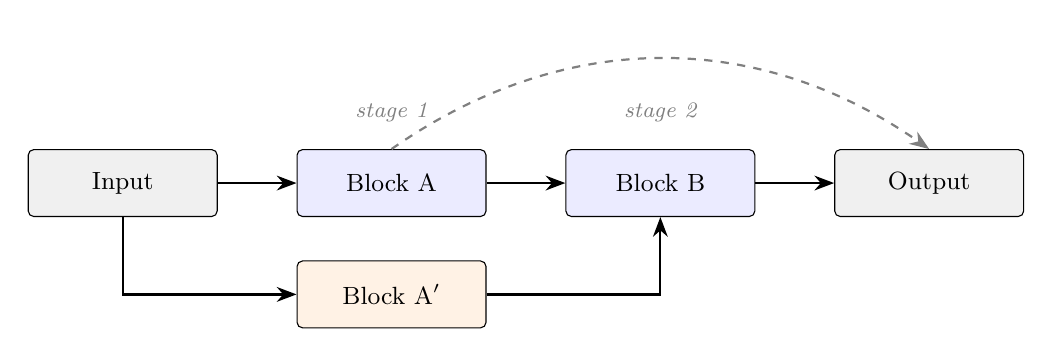
\begin{tikzpicture}[node distance=0.55cm and 1.0cm]

\node[io] (in) {Input};
\node[stage, right=of in] (a) {Block A};
\node[stage, right=of a] (b) {Block B};
\node[io, right=of b] (out) {Output};

\draw[flow] (in) -- (a);
\draw[flow] (a) -- (b);
\draw[flow] (b) -- (out);

\node[alt, below=of a] (ap) {Block A$'$};
\draw[flow] (in.south) |- (ap.west);
\draw[flow] (ap.east) -| (b.south);

\draw[skip] (a.north) to[out=35, in=145] (out.north);

\node[layer, above=0.22cm of a] {stage 1};
\node[layer, above=0.22cm of b] {stage 2};

\end{tikzpicture}
\end{document}
